\documentclass[tikz,border=4pt]{standalone}
\begin{document}
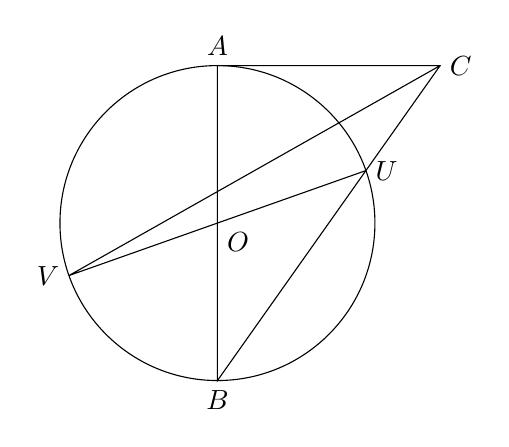
\begin{tikzpicture}
\coordinate (O) at (0,0);\coordinate (A) at (0,2);\coordinate (B) at (0,-2);\coordinate (C) at ({2*sqrt(2)},2);\coordinate (U) at ({4*sqrt(2)/3},{2/3});\coordinate (V) at ({-4*sqrt(2)/3},{-2/3});\draw (O) circle (2);\draw (A)--(B)--(C)--(A) (V)--(U) (V)--(C);\node[above] at (A) {$A$};\node[below] at (B) {$B$};\node[below right] at (O) {$O$};\node[right] at (C) {$C$};\node[right] at (U) {$U$};\node[left] at (V) {$V$};
\end{tikzpicture}
\end{document}
